\section{Konzeptbeschreibung}

\subsection{Systembeschreibung}
Das System besteht zentral aus einem Mikrokontroller, welcher sich über Bluetooth mit einer App auf dem Smartphone verbinden kann. Von dieser App erhält der Mikrokontroller GPS-Koordinaten, welche er dank eines eigenen GPS-Sensors vergleichen kann. Über einen Kompass und diese beiden Koordinatensätze ist das System in der Lage die verbauten Motoren so anzusteuern, dass die Distanz zwischen den beiden Koordinatensätze sich verringert. \\
\\
Des Weiteren verfügt das System über eine Box, welche für mindestens 12 Bierdosen à 0.5L Platz hat und diese aktiv kühlt.\\
\\
Die Energieversorgung wird über eine verbaute Batterie und eine Custom-Spannungsversorgung gewährleistet.\\
\\
Über eine Bluetooth Verbindung soll der Roboter GPS Koordinaten vom Smartphone erhalten. Er soll eine Distanz und einen Winkel zwischen diesen GPS-Koordinaten und denen des sich an Bord befindenden Sensors errechnen. Über den Kompass soll er stets die eigene Ausrichtung kennen und den errechneten Winkel in Relation setzen. Durch kontinuierliche Wiederholung dieses Prozesses soll der Roboter in der Lage sein, sich dem Smartphone anzunähern.\\
\\
Davon unabhängig soll sich die Kühlbox von der Batterie aus mit Strom versorgen und die ausreichende Kühlung der Getränke sicherstellen. Dieser Prozess findet ohne Überwachung statt.

\subsection{Grundsätzlicher Aufbau (Blockschaltbild)}
\begin{figure}[H]
    \begin{center}
    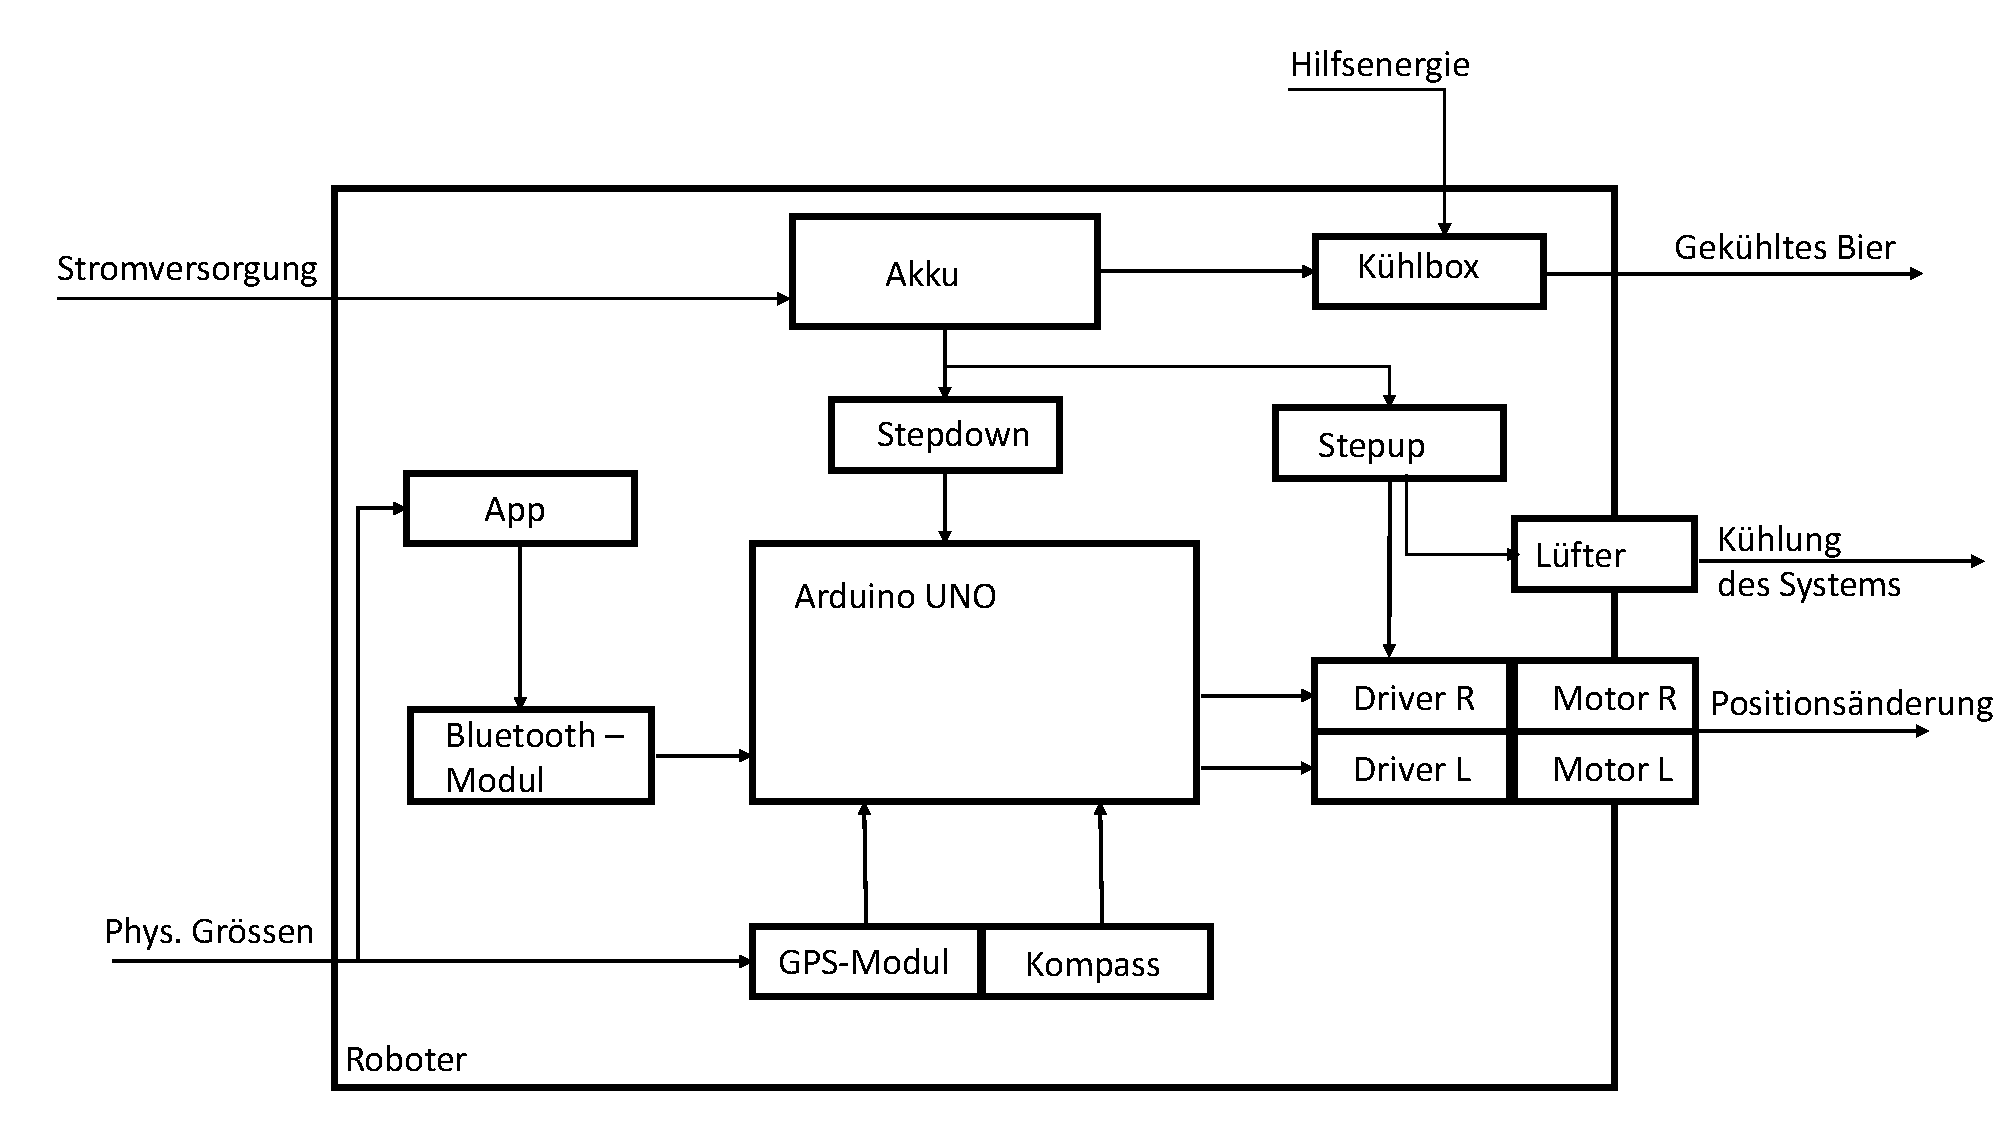
\includegraphics[width=\linewidth]{blockdiagramm.pdf}
    \end{center}
    \caption{Blockschaltbild}
\end{figure}

\subsection{Use-Case Übersicht}
\begin{figure}[H]
    \begin{center}
    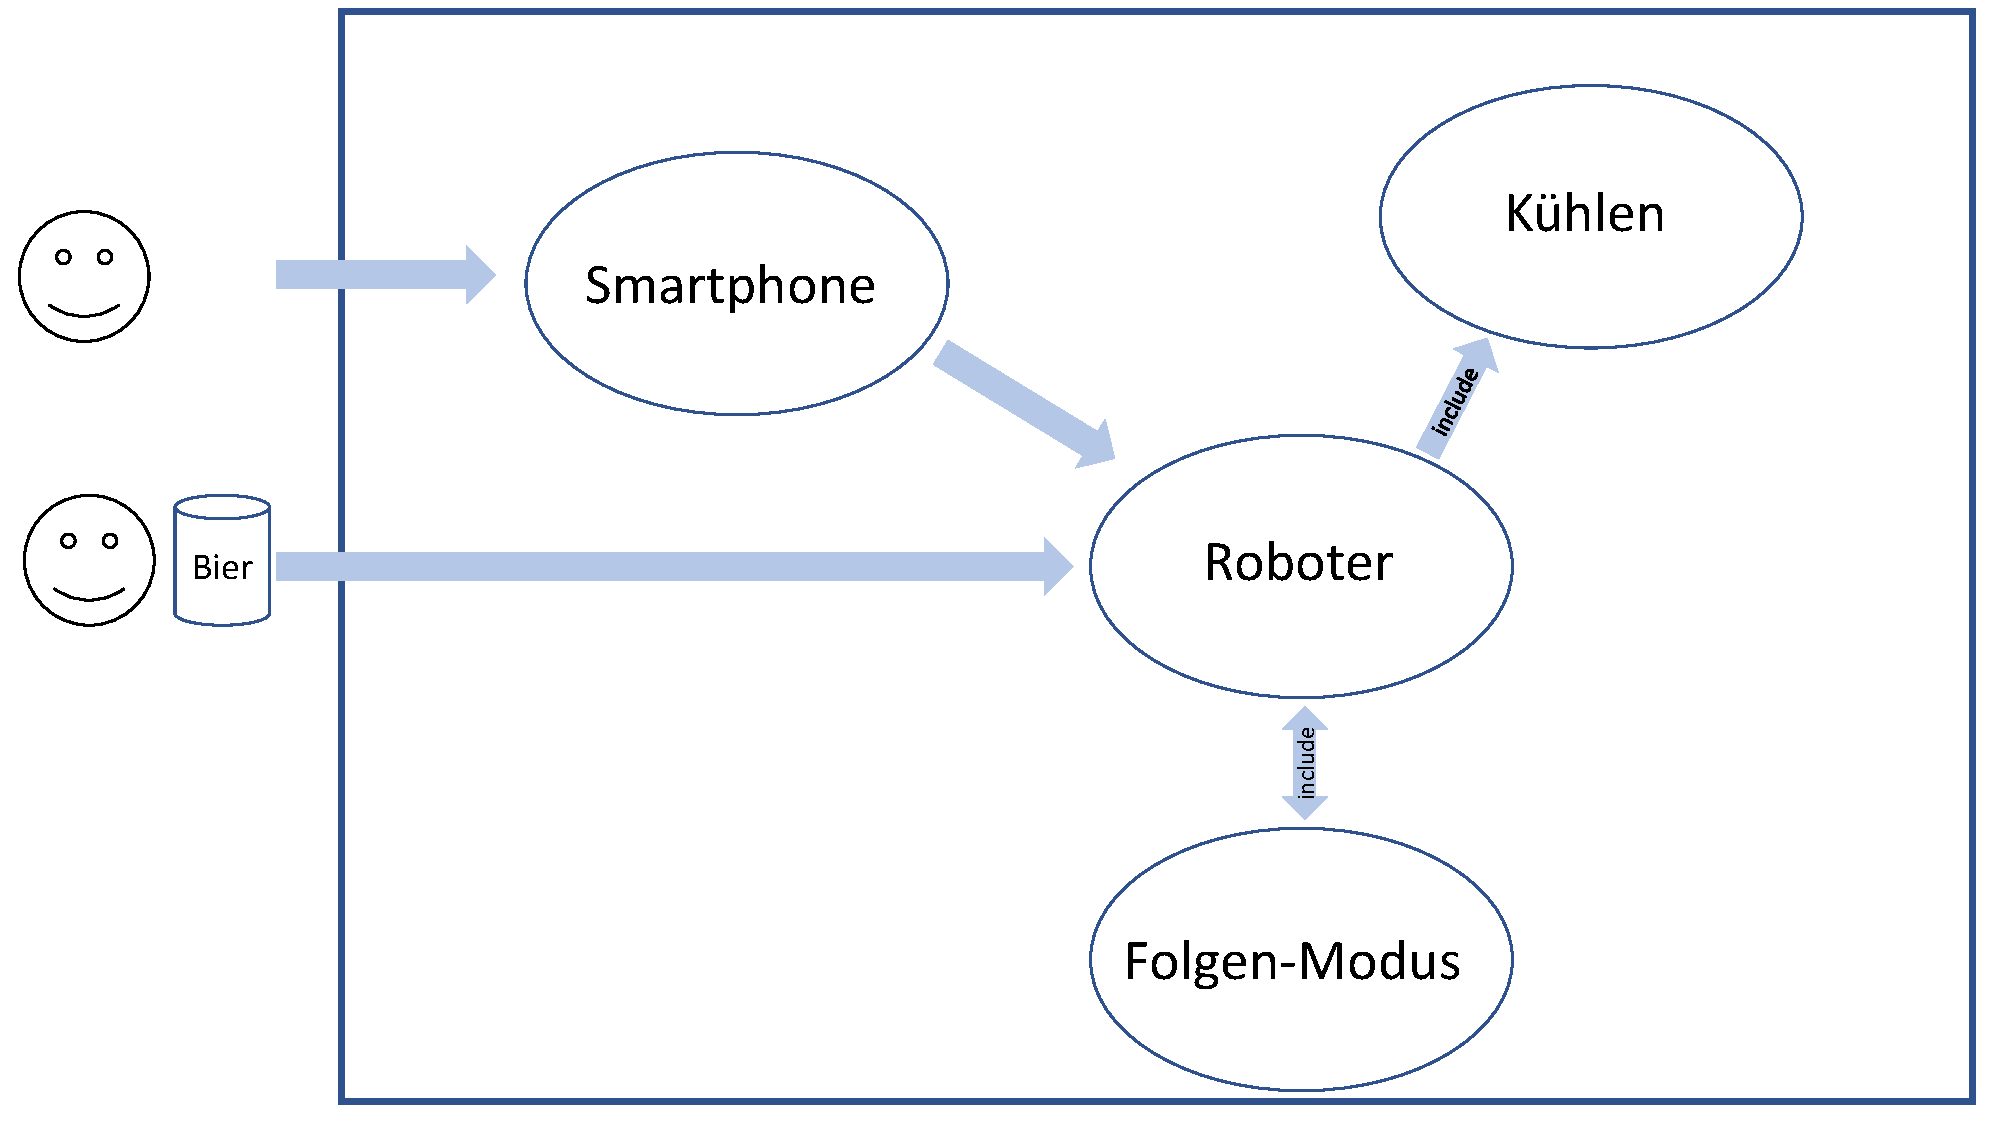
\includegraphics[width=\linewidth]{Use_case_diagramm.pdf}
    \end{center}
    \caption{Use-Case Diagramm}
\end{figure}

% Please add the following required packages to your document preamble:
% \usepackage{graphicx}
\begin{table}[H]
    \centering
    \caption{Use-Case Übersicht}
    \label{tab:my-table}
    \resizebox{\textwidth}{!}{%
    \begin{tabular}{|l|l|l|}
    \hline
    Nr. &
      Titel &
      Beschreibung \\ \hline
      \rule{0pt}{25pt} 1 &
      Folgen-Modus &
      \parbox{14cm}{Der Benutzer kann über eine Applikation auf seinem Smartphone den Folgen-Modus \\ aktivieren und deaktivieren, wodurch der Roboter dem Smartphone des Benutzers \\ folgt.} \\ \hline
      \rule{0pt}{25pt} 2 &
      Kühlen &
      \parbox{14cm}{Der User kann mindestens 12 Bierdosen in der Kühlbox platzieren und diese mit \\ deutlich unter Lufttemperatur wieder aus der Kühlbox entnehmen.} \\ \hline
    \end{tabular}%
    }
    \end{table}


\subsection{Vergleich mit bestehenden Lösungen}
Es existiert bereits mindestens ein solches, sehr gut dokumentiertes Projekt, an welchem wir uns orientiert haben. Es soll aber kein kompletter Nachbau werden, weshalb unter anderem die aktive Kühlfunktion integriert wurde.

\pagebreak

\subsection{Nicht-funktionale Anforderungen}
Mit Bezug auf die Bedienbarkeit soll das ganze System intuitiv bedienbar sein.\\
\\
Bei der Leistung soll mit vollgeladenem Akku der Roboter 3 Stunden kühlen und eine Stunde fahren können.\\
\\
In Betrachtung der Sicherheit und Zuverlässigkeit ist Sämtliche Elektronik-Komponenten vor Witterung, Sonneneinstrahlung und Überhitzung geschützt. Stromschläge werden dadurch vermieden, dass nur Niederspannungs-Komponenten ohne Schwierigkeiten mit blossen Fingern erreichbar sein sollen. Ein Hauptschalter soll ausserdem in der Lage sein die Stromzufuhr zum gesamten System zu unterbrechen.
